%%
%% 2019 07 04 Ph. G. Freimann
%%

\section{Lineare Gleichungen mit Parametern}\index{Gleichungen!lineare mit Parametern}\index{Parameter}
\sectuntertitel{Alle Zahlen sind gleich; nur einige sind gleicher.}
\theorieTALS{89}{2.2.2}
\theorieGESO{116}{8.2}
%%%%%%%%%%%%%%%%%%%%%%%%%%%%%%%%%%%%%%%%%%%%%%%%%%%%%%%%%%%%%%%%%%%%%%%%%%%%%%%%%
\subsection*{Lernziele}

\begin{itemize}
\item Lineare Gleichungen mit Parametern
\end{itemize}

Parameter = (wörtlich) «Neben-Maß»

Griechisch $\pi\alpha\rho\alpha$ (para), deutsch: ‚neben‘ und $\mu\epsilon\tau\rho\omega\nu$ (metron) deutsch: ‚Maß‘


\TALS{%% TALS Schieberegler im CAS-Rechner

\paragraph{Schieberegler}\index{Schieberegler} Der Taschenrechner \textit{TI-$n$Spire CX
  II-T CAS} kann Terme in der Variablen $x$ parametrisiert
darstellen. Erstellen Sie dazu in einem Dokument eine
\textit{notes}-Page und definieren Sie den Term $terma := a\cdot
x+0.5$. In einem neuen Grafik-Fenster (Page) zum selben Problem
definieren Sie die Funktion $f1(x):=terma$. Damit erscheint die Frage
nach einem Schieberegler, welcher uns den Parameter $a$ verändern
lassen kann.

\bbwCenterGraphic{6cm}{allg/gleichungen/img/LineareFunktionTR_terma.png}
%  \begin{center}
%   \raisebox{-1cm}{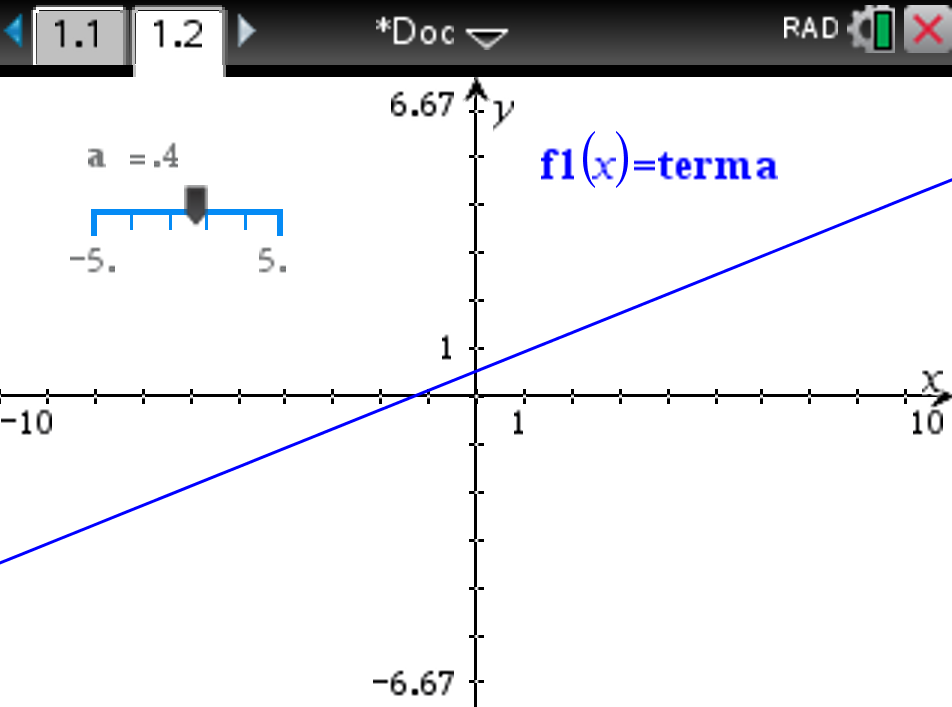
\includegraphics[width=6cm]{img/LineareFunktionTR_terma.png}}
%  \end{center}


\paragraph{Frage 1} Bei welchem Parameter $b$ hat die folgende Gleichung für $x$ die Lösung $1.5$?
$$-2x + b = 0$$

\noTRAINER{$$.....................................$$}
\TRAINER{$$b = 3$$}
Dies lösen wir, indem wir die gesuchte Lösung für $x$ einsetzen und nach $b$ auf"|lösen. Graphisch kann dies auch mit dem CAS-Rechner \textit{gelöst} werden. Definieren Sie «termb := $-2\cdot{}x+b$» und zeichnen Sie den Graphen in einer Graph-Page.
Erstellen Sie einen «Slider»\index{Slider}\index{Schieberegler} für $b$ und ziehen Sie an
diesem \textit{Slider}, bis der Wert der Geraden auf der $x$-Achse den
Wert 1.5 (gesuchte Lösung) angenähert hat.


\paragraph{Frage 2} Bei welchem Parameter $b$ hat die folgende Gleichung für $x$ die Lösung $1.5$?
$$ax-3=0$$

\noTRAINER{$$.....................................$$}
\TRAINER{$$a=2$$}
Dies nähern wir auch mit dem CAS-Rechner an. Definieren Sie den Term
$terma$ neu ($terma := a\cdot{}x-3$) und zeichnen Sie den Graphen in einer Graph-Page.
Ziehen Sie am \textit{Slider}, bis der Wert der Geraden auf der
$x$-Achse dem Wert 1.5 (gesuchte Lösung) genug nahe kommt.
}


\TALS{Aufg 247 l aus \cite{frommenwiler17alg}}

\TALS{\noTRAINER{\noteLines{17}}}
\TALS{\TRAINER{Vorzeigeaufgabe
  $$\frac{x}{n} + a - \frac{x}{m} + b = mx + c$$
  Lösungsweg:
  $$ \cdot n      \rightarrow x + an - \frac{nx}{m} + bn = mnx + cn$$
  $$ \cdot m      \rightarrow mx + anm - nx + bnm = nm^2x + cnm$$
  $$ x \textrm{\, nach links}  \rightarrow mx - nx -nm^2x = cnm -anm - bnm$$
  $$ x \textrm{\, ausklammern} \rightarrow x(m - n -nm^2) = cnm -anm - bnm$$
  $$ \textrm{\, dividieren}    \rightarrow x = \frac{cnm - anm - bnm}{m-n-nm^2} = \frac{nm(c-a-b)}{m-n-nm^2}$$
}}

\GESO{\TNT{5.2}{Vorzeigeaufgabe
  Aufg Beispiel 1 S. 117 \cite{marthaler17})
  $$(x-b)(x+a)-b=(b-x)(a-x)$$
  Lösungsweg:\\
  Termumformung: $x^2 + ax-bx-ab-b=ab-bx-ax+x^2$\\
  $-x^2+b+bx-ax-ab$ (alle x nach links): $\rightarrow ax-bx+bx+ax=ab+ab+b$\\
  Termumformung: $2ax=2ab+b$\\
  $: 2a$ (alle nicht x nach rechts): $\rightarrow x=\frac{2ab+b}{2a}$\\
}}


\subsection*{Aufgaben}
\TALS{\aufgabenfarbe{Aufgaben: \cite{frommenwiler17alg} S. 89, Aufg. 246. a) 247. a)
  c) g) 248. a) d) i) 249.}}

\TALS{Textaufgaben: \cite{frommenwiler17alg} S. 89 Aufg. 253}

\GESO{\aufgabenfarbe{Aufgaben: \cite{marthaler17} Seite 128: 7. a) b) c) e)
  8.  a) d) e) f)
  9. a) b) c) e) f)
  10. a) b)
}}
\newpage
